\documentclass[12pt]{article}

%Allgemeine Einstellungen

%Abstände
\usepackage[a4paper,left=3cm,right=3cm,top=3cm,bottom=3.5cm,headsep=12pt]{geometry}%Bottom extra 0.5cm für Footer

%Deutsches Sprachpacket
\usepackage[german,ngerman]{babel}

%Times New Roman
\usepackage{mathptmx}

%Titelseite einbinden
\usepackage{pdfpages}

%1.5-Zeilenabstand
\usepackage[onehalfspacing]{setspace}

%Stil der Überschriften, siehe ueberschriften.sty
\usepackage[numeric]{ueberschriften}

%Stil des Inhaltsverzeichnisses, siehe inhaltsverzeichnis.sty
\usepackage[numeric]{inhaltsverzeichnis}

%Abkürzungsverzeichnis, siehe abk_verzeichnis.sty
\usepackage{abk_verzeichnis}

%Stil der Fußzeilen, siehe fusszeilen.sty
\usepackage{fusszeilen}

%Literaturverzeichnis und Zitate, siehe literatur.sty
\usepackage{literatur}

%Stil für Header und Footer, siehe header_footer.sty
%Wenn nicht erwünscht, müssen auch die Befehle \frontmatter, \mainmatter auskommentiert werden
\usepackage{header_footer}

%Stile für Code-Ausschnitte, siehe codes.sty
\usepackage{codes}

%Stile für Anhänge, Bilder, ...
\usepackage{anhang}

%Silbentrennung (manche Worte werden am Zeilenende nicht getrennt, diese müssen dann nachgetragen werden)
\usepackage[T1]{fontenc}
\hyphenation{öf-fent-lich-en}

%DEBUGGING (Zeigt Boxen an)
%\usepackage{showframe}
\setlength{\skip\footins}{12pt}

\usepackage{makecell}
\usepackage{placeins}

\usepackage{titletoc}
\usepackage{chngcntr}
\newcounter{mysection}
\titleclass{\mysection}{straight}[\part]
\titleformat{\mysection}[hang]
  {\normalfont\LARGE\bfseries}{\thesubparagraph .\themysection}{1em}{}
\titlespacing*{\mysection}{0pt}{3.5ex plus 1ex minus .2ex}{2.3 ex plus .2ex}
\renewcommand{\themysection}{\arabic{mysection}}
\counterwithin{subparagraph}{mysection}

\titlecontents*{mysection}[2em]{}{\bfseries\contentslabel{2em}}{}
{\titlerule*[.5pc]{.}\contentspage}[]
\dottedcontents{section}[4em]{}{2em}{.5pc}

\begin{document}

\renewcommand{\mytitle}{Dokumentation/Tutorial}%Titel für oben links
\renewcommand{\myauthor}{Dr. Frank N. Furter}%Name für unten links

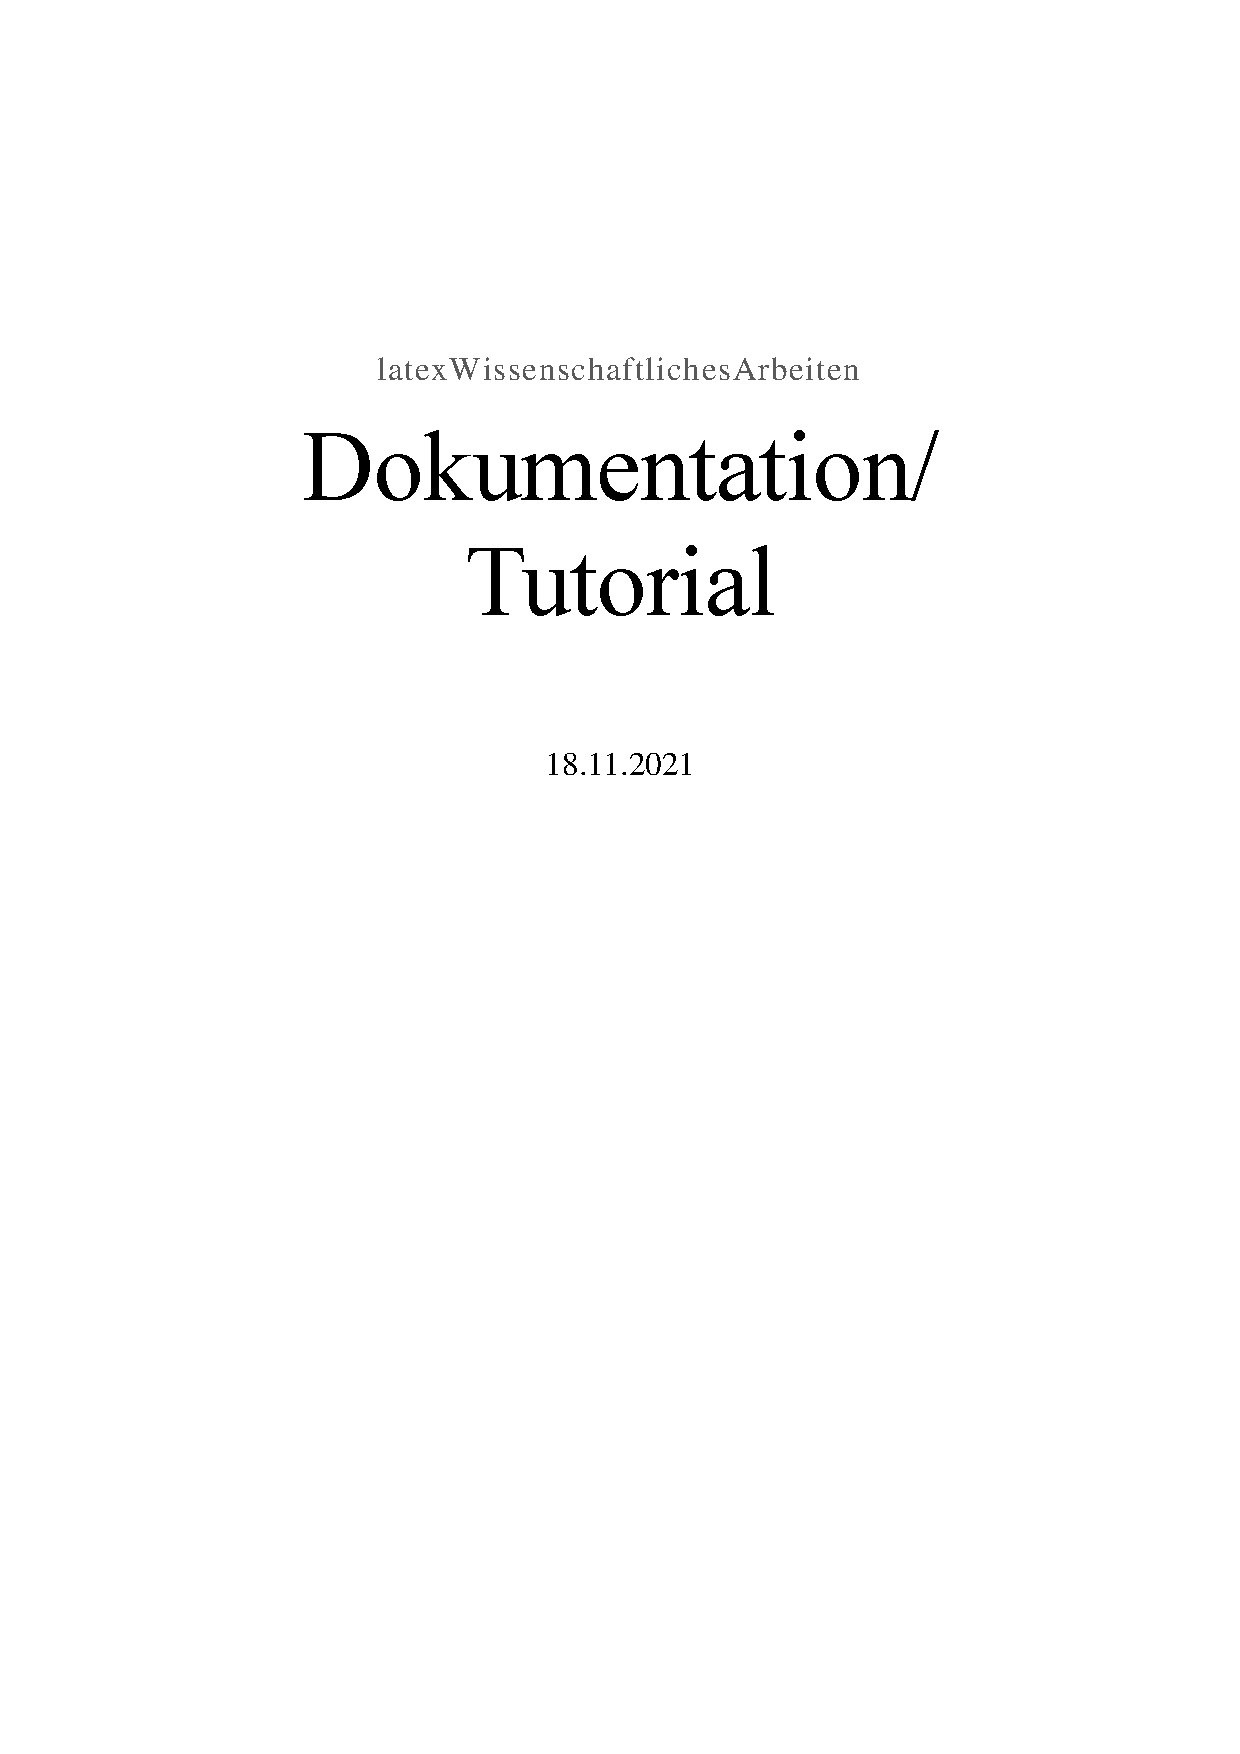
\includepdf[pages={1-}]{titelseiteAlternative.pdf}

\frontmatter%Stil des Headers/Footers ändern

\pagenumbering{Roman}

\addcontentsline{toc}{part}{Abkürzungsverzeichnis}%Abk-Verz. ins Inhaltsverzeichnis
\printabbreviations%abk_verzeichnis.sty
\clearpage
\renewcommand{\plaintitle}{Abbildungsverzeichnis}
\addcontentsline{toc}{part}{Abbildungsverzeichnis}
{\def\makebox[#1][#2]#3{#3}%
\listoffigures
}
\clearpage
\renewcommand{\plaintitle}{Tabellenverzeichnis}
\addcontentsline{toc}{part}{Tabellenverzeichnis}
{\def\makebox[#1][#2]#3{#3}%
\listoftables
}
\clearpage
\renewcommand{\plaintitle}{Inhaltsverzeichnis}%Titel für oben Rechts
%Defbox, damit gepunktete Linie bis zur Zahl geht
{\def\makebox[#1][#2]#3{#3}%
	\tableofcontents
}

\addtocontents{toc}{\vspace{24pt}}%Freiraum im ToC

\clearpage
\mainmatter%Stil des Headers/Footers ändern
\pagenumbering{arabic}

\part{Vorwort}
In dieser Doku wird der Aufbau und die Funktionsweise dieser Vorlage und der dahinter stehenden Mechanismen erläutert. Ein grundlegendes Verständnis von \textit{LaTeX} wird vorausgesetzt. Diese Doku wurde mithilfe der Vorlage erstellt.
\part{Dokumentenstruktur}
Die Struktur kann bis zu sechs Kapitelebenen umfassen.
\section{test}
hallo
\subsection{test1}
hallo
\subsubsection{test11}
hallo
\paragraph{test111}
hallo
\subparagraph{test1111}
hallo
\mysection{test111111}
hallo

\clearpage
\frontmatter%Stil des Headers/Footers ändern
\renewcommand{\plaintitle}{Literaturverzeichnis}
\pagenumbering{Roman}
\setcounter{page}{5}
\addtocontents{toc}{\vspace{24pt}}
\addcontentsline{toc}{part}{Literaturverzeichnis}%Literatur-Verz. ins Inhaltsverzeichnis
\printMyBibliography

\end{document}